\section{Introduction}
\label{sec:intro}

\begin{figure}
  \begin{subfigure}[b]{\columnwidth}
    \centering
    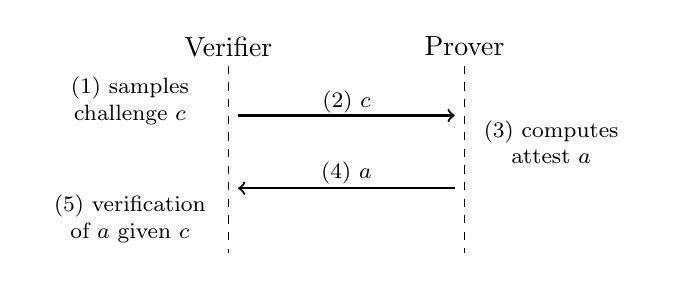
\begin{tikzpicture}[
	squarednode/.style={rectangle, draw=black, thick, minimum size=10mm},
	invisiblenode/.style={rectangle, draw=white}
]
	%Nodes
	\node (verifier) at (0.5,2) {Verifier};
	\node[invisiblenode] (1) at (0.5,1) {};
	\node[invisiblenode] (2) at (0.5,0.2) {};
	\node[invisiblenode] (3) at (0.5,-.75) {};
	
	\node (prover) at (3.5,2) {Prover};
	\node[invisiblenode] (4) at (3.5,1) {};
	\node[invisiblenode] (5) at (3.5,0.2) {};
	\node[invisiblenode] (6) at (3.5,-.75) {};
	
	\node[invisiblenode](sample) at (-0.75,1.3) 
		   {\footnotesize\begin{tabular}{c}(1) samples \\challenge $c$\end{tabular}};
		   \node[invisiblenode](nonce) at (2,1.3) 
		        {\footnotesize(2) $\boldsymbol{c}$};
		        \node[invisiblenode](attest) at (4.6,.75) 
		             {\footnotesize\begin{tabular}{c} (3) computes \\ attest $\boldsymbol{a}$ \end{tabular}};
		             \node[invisiblenode](reply) at (2,0.4) 
		                  {\footnotesize(4) $\boldsymbol{a}$};
		                  \node[invisiblenode](verify) at (-0.75,-0.2)
		                       {\footnotesize\begin{tabular}{c} (5) verification \\ of $\boldsymbol{a}$ given $\boldsymbol{c}$ \end{tabular}};
		                       
		                       %Lines
		                       \draw[dashed]    (verifier.south) -- (3.north);
		                       \draw[dashed]    (prover.south)   -- (6.north);
		                       \draw[->, thick] (1.north east)   -- (4.north west);
		                       \draw[<-, thick] (2.east)         -- (5.west);
		                       
\end{tikzpicture}



    \caption{Protocol}
    \label{fig:problem:prot}
  \end{subfigure}
\\
\\
  \begin{subfigure}[b]{\columnwidth}
    \centering
	  \section{Problem Formulation} \label{sec:probdef}

This section formally defines the problem of restoring a given pruned network with only using its original pretrained CNN in a way free of data and fine-tuning.



% Unlike many existing works utilize data for identifying unimportant filters as well as fine-tuning to this end, we cannot evaluate the filter importance by data-dependent values like activation maps (\textit{a.k.a.} channels) as our focus in this paper is not to use any training data. Thus, in our problem setting, we can only exploit the values of filters in the original network, and thereby have to make some changes in the remaining filters of the pruned network so that the network can return the output not too much different from the original one.

% No matter how much we carefully select unimportant filters to be pruned, some kinds of retraining process appears inevitable as done by the most existing works to this end. However, since our focus in this paper is not to use any training data, we cannot evaluate the importance of filters by data-dependent values like activation maps (\textit{a.k.a.} channels). 

% To this end, they not only use a careful criterion (\textit{e.g.}, L1-norm), but also fine-tune the network using the original data.
% Most of filter pruning methods try to select filters to be pruned prudently so that pruned network's output be similar to the original network's. To this end, they prune the unimportant filters and then fine-tune the pruned network with using the train data. 

% How can we restore the the pruned networks without any data? In other words, it implies that we cannot use any data-driven values(i.e., activation maps) and we can only exploit the values of original filters. In that case, the only thing we can do maybe changing the weights of remained filters appropriately not to amplify the difference between pruned and unpruned network's outputs through the information of original filters.

\begin{figure*}[t]
	\centering
    \subfigure[\label{fig:matrix:a}Pruning matrix]{\hspace{6mm}\includegraphics[width=0.35\columnwidth]{./figure/LBYL_figure_2_1.pdf}\hspace{6mm}} 
    \subfigure[\label{fig:matrix:b}Delivery matrix for LBYL]{\hspace{6mm}\includegraphics[width=0.35\columnwidth]{./figure/LBYL_figure_2_2.pdf}\hspace{6mm}}
    \subfigure[\label{fig:matrix:c}Delivery matrix for one-to-one]{\hspace{9mm}\includegraphics[width=0.35\columnwidth]{./figure/LBYL_figure_2_3.pdf}\hspace{9mm}} 
    \caption{Comparison between pruning matrix and delivery matrix, where the $4$-th and $6$-th filters are being pruned among $6$ original filters}
	\label{fig:matrix}
	\vspace{-2mm}
\end{figure*}



\subsection{Filter Pruning in a CNN}
Consider a given CNN to be pruned with $L$ layers, where each $\ell$-th layer starts with a convolution operation on its input channels, which are the output of the previous $(\ell-1)$-th layer $\mathbf{A}^{(\ell-1)}$, with the group of convolution filters $\mathbf{W}^{{(\ell)}}$ and thereby obtain the set of \textit{feature maps} $\mathbf{Z}^{(\ell)}$ as follows:
\begin{equation}
\boldsymbol{\mathbf{Z}}^{(\ell)} = {\mathbf{A}^{(\ell-1)} \circledast {\mathbf{W}}^{(\ell)}},
\nonumber
\end{equation}
where $\circledast$ represents the convolution operation. Then, this convolution process is normally followed by a batch normalization (BN) process and an activation function such as ReLU, and the $\ell$-th layer finally outputs an \textit{activation map} $\mathbf{A}^{(\ell)}$ to be sent to the $(\ell+1)$-th layer through this sequence of procedures as:
\begin{equation}
\mathbf{A}^{(\ell)} = \F(\N(\mathbf{Z}^{(\ell)})),
\nonumber
\end{equation}
where $\F(\cdot)$ is an activation function and $\N(\cdot)$ is a BN procedure.

Note that all of $\mathbf{W}^{(\ell)}$, $\mathbf{Z}^{(\ell)}$, and $\mathbf{A}^{(\ell)}$ are tensors such that: $\mathbf{W}^{(\ell)} \in \mathbb{R}^{m \times n \times k \times k}$ and $\mathbf{Z}^{(\ell)},\mathbf{A}^{(\ell)} \in \mathbb{R}^{m \times w \times h}$, where (1) $m$ is the number of filters, which also equals the number of output activation maps, (2) $n$ is the number of input activation maps resulting from the $(\ell-1)$-th layer, (3) $k \times k$ is the size of each filter, and (4) $w \times h$ is the size of each output channel for the $\ell$-th layer.

\smalltitle{Filter pruning as n-mode product}
When filter pruning is performed at the $\ell$-th layer, all three tensors above are consequently modified to their \textit{damaged} versions, namely $\mathbf{\Tilde{W}}^{(\ell)}$, $\mathbf{\Tilde{Z}}^{(\ell)}$, and $\mathbf{\Tilde{A}}^{(\ell)}$, respectively, in a way that: $\mathbf{\Tilde{W}}^{(\ell)} \in \mathbb{R}^{t \times n \times k \times k}$ and $\mathbf{\Tilde{Z}}^{(\ell)},\mathbf{\Tilde{A}}^{(\ell)} \in \mathbb{R}^{t \times w \times h}$, where $t$ is the number of remaining filters after pruning and therefore $t < m$. Mathematically, the tensor of remaining filters, \textit{i.e.}, $\mathbf{\Tilde{W}}^{(\ell)}$, is obtained by the \textit{$1$-mode product} \cite{DBLP:journals/siamrev/KoldaB09} of the tensor of the original filters $\mathbf{W}^{(\ell)}$ with a \textit{pruning matrix} $\boldsymbol{\S} \in \mathbb{R}^{m \times t}$ (see Figure \ref{fig:matrix:a})
as follows:
\begin{eqnarray}\begin{split}\label{eq:pruning}
\mathbf{\Tilde{W}}^{(\ell)} = {\mathbf{W}}^{(\ell)} \times_{1} {\boldsymbol{\S}}^{T},\text{where }\boldsymbol{\S}_{i,k} = 
  \begin{cases} 
   1~ \text{if } i = i'_k \\
   0~ \text{otherwise}
  \end{cases} \\
  \text{s.t. } i, i'_k \in [1, m] 
  \text{ and } k \in [1, t].
  \end{split}
\end{eqnarray}
  
By Eq. (\ref{eq:pruning}), each $i'_k$-th filter is not pruned and the other $(m-t)$ filters are completely removed from $\mathbf{W}^{(\ell)}$ to be $\mathbf{\Tilde{W}}^{(\ell)}$.

This reduction at the $\ell$-th layer causes another reduction for each filter of the $(\ell+1)$-th layer so that $\mathbf{W}^{(\ell+1)}$ is now modified to $\mathbf{\Tilde{W}}^{(\ell+1)} \in \mathbb{R}^{m' \times t \times k' \times k'}$, where $m'$ is the number of filters of size $k' \times k'$ in the $(\ell+1)$-th layer. Due to this series of information losses, the resulting feature map (\textit{i.e.}, $\mathbf{Z}^{(\ell+1)}$) would severely be damaged to be $\mathbf{\Tilde{Z}}^{(\ell+1)}$ as shown below:
\begin{equation}
{\mathbf{\Tilde{Z}}}^{{(\ell+1)}} = \mathbf{\Tilde{A}}^{(\ell)} \circledast {\mathbf{\Tilde{W}}}^{(\ell+1)}~~~\not\approx~~~\mathbf{Z}^{(\ell+1)}
\label{eq:eq}\nonumber
\end{equation}
The shape of $\mathbf{\Tilde{Z}}^{(\ell+1)}$ remains the same unless we also prune filters for the $(\ell+1)$-th layer. If we do so as well, the loss of information will be accumulated and further propagated to the next layers. Note that $\mathbf{\Tilde{W}}^{(\ell+1)}$ can also be represented by the \textit{$2$-mode product} \cite{DBLP:journals/siamrev/KoldaB09} of $\mathbf{W}^{(\ell+1)}$ with the transpose of the same matrix $\boldsymbol{\S}$ as:
\begin{equation} \label{eq:pruning2}
\mathbf{\Tilde{W}}^{(\ell+1)} = {\mathbf{W}}^{(\ell+1)} \times_{2} {\boldsymbol{\S}^T}
\end{equation}




\subsection{Problem of Restoring a Pruned Network without Data and Fine-Tuning}
As mentioned earlier, our goal is to restore a pruned and thus damaged CNN without using any data and re-training process, which implies the following two facts. First, we have to use a pruning criterion exploiting only the values of filters themselves such as L1-norm. In this sense, this paper does not focus on proposing a sophisticated pruning criterion but intends to recover a network somehow pruned by such a simple criterion. Secondly, since we cannot make appropriate changes in the remaining filters by fine-tuning, we should make the best use of the original network and identify how the information carried by a pruned filter can be delivered to the remaining filters.

% For brevity, we formulate our problem here with respect to a specific layer, say $\ell$, and then it can trivially be generalized for the entire network. 
\smalltitle{Delivery matrix}
In order to represent the information to be delivered to the preserved filters, let us first think of what the pruning matrix $\boldsymbol{\S}$ means. As defined in Eq. (\ref{eq:pruning}) and shown in Figure \ref{fig:matrix:a}, each row is either a zero vector (for filters being pruned) or a one-hot vector (for remaining filters), which is intended only to remove filters without delivering any information. Intuitively, we can transform this pruning matrix into a \textit{delivery matrix} that carries information for filters being pruned by replacing some meaningful values with some of the zero values therein. Once we find such an \textit{ideal} $\boldsymbol{\S^*}$, we can plug it into $\boldsymbol{\S}$ of Eq. (\ref{eq:pruning2}) to deliver missing information propagated from the $\ell$-th layer to the filters at the $(\ell+1)$-th layer, which will hopefully generate an approximation $\mathbf{\hat{Z}}^{(\ell+1)}$ close to the original feature map as follows:
\begin{equation} \label{eq:fmap_approx}
{\mathbf{\hat{Z}}}^{{(\ell+1)}} = {\mathbf{\Tilde{A}}^{(\ell)} \circledast ({\mathbf{W}}^{(\ell+1)} \times_{2} {\boldsymbol{\S^*}^T})}
~~~\approx~~~\mathbf{Z}^{(\ell+1)}
\end{equation}
Thus, using the delivery matrix $\boldsymbol{\mathcal{S^*}}$, the information loss caused by pruning at each layer is recovered at the feature map of the next layer.

\smalltitle{Problem statement}
Given a pretrained CNN, our problem aims to find the best delivery matrix $\boldsymbol{\mathcal{S^*}}$ for each layer without any data and training process such that the following \textit{reconstruction error} is minimized:
\begin{equation}
\sum\limits_{i = 1}^{m'}\|{{\mathbf{Z}}_{i}^{{(\ell+1)}}-{\hat{\mathbf{Z}}}_{i}^{{(\ell+1)}}}\|_1,
\label{eq:goal}
\end{equation}
where ${\mathbf{Z}}_i^{{(\ell+1)}}$ and ${\hat{\mathbf{Z}}}_i^{{(\ell+1)}}$ indicate the $i$-th original feature map and its corresponding approximation, respectively, out of $m'$ filters in the $(\ell+1)$-th layer. Note that what is challenging here is that we cannot obtain the activation maps in $\mathbf{A}^{(\ell)}$ and $\mathbf{\Tilde{A}}^{(\ell)}$ without data as they are data-dependent values.

% = \sum\limits_{i = 1}^{m'}\|{{\mathbf{Z}}_{i}^{{(\ell+1)}}-{\mathbf{\Tilde{A}}^{(\ell)} \circledast ({\mathbf{W}}^{(\ell+1)} \times_{2} {\boldsymbol{\mathcal{S^*}^T}})}}\|_{1}


% Our goal is finding the approximation matrix $\boldsymbol{\mathcal{S}}$ to minimize the reconstruction error between the pruned model and the original model without any data, and effectively deliver missing information for pruned filters using this approximation matrix


% $\testit{s}$,which can be represented as below.

% \begin{equation}
% \boldsymbol{\mathcal{S}} =  \underset{{\boldsymbol{\mathcal{S}}}}{\mathrm{argmin}} \sum\limits_{{i} = 1}^{m_{\ell+1}} \|{{\mathbf{Z}}_{i,:,:}^{{(\ell+1)}}-{\hat{\mathbf{Z}}}_{i,:,:}^{{(\ell+1)}}}\|_{1} 
% \label{eq:eq1}
% \end{equation}



% Let us first recall that the ultimate goal of network pruning is to make the output of a pruned network as close as possible to that of its original network. Unlike many existing pruning methods, our focus is not to use any training data at all for the entire pruning and recovery process, and this implies the following two facts. First, we cannot evaluate the filter importance by data-dependent values like activation values or gradients, but have to use a pruning criterion exploiting only the values of filters themselves such as L1-norm. Furthermore, instead of fine-tuning with data, the only thing we can do for the pruned network is to make appropriate changes in the remaining filters by identifying some relationships between pruned filters and the other preserved ones without any support from data. Based on this intuition, this section mathematically and generally defines the problem of restoring a pruned neural network in a manner free of data and fine-tuning.


% Thus, we make approximation matrix $\testit{s}$ $\in$ $\mathbb{R}^{m_{\ell} \times t_{\ell}}$ with relationship between the pruned filter and preserved filters in $\ell$-th layer and then apply it to the original filters in $(\ell+1)$-th layer to compensate for pruned feature maps $\boldsymbol{\hat{\mathbf{Z}}}^{{(\ell+1)}}$ as shown below.
% (\textit{i.e.}, Let $\hat{\mathbf{W}}^{(\ell+1)}$ be ${\mathbf{W}}^{(\ell+1)}$ $\times_2$ ${{\textit{s}}} $, where $\times_2$ is 2-mode matrix product) 

% \begin{equation}
% \mathbf{Z}^{(\ell+1)} = {\mathbf{A}}^{(\ell)} \circledast {\mathbf{W}}^{(\ell+1)}
% \approx {\hat{\mathbf{A}}^{(\ell)} \circledast ({\mathbf{W}}^{(\ell+1)} \times_{2} {{s}}) = {\hat{\mathbf{Z}}}^{{(\ell+1)}}}
% \label{eq:eq}\nonumber
% \end{equation}




% For a Convolutional Neural Network (CNN) with $L$ layers, we denote $\mathcal{A}{^{(\ell-1)}}$ $\in$ $\mathbb{R}^{n_{\ell -1 } \times h_{\ell -1} \times w_{\ell -1}}$ is activation maps at $\ell-1$-th layer, where $n_{\ell -1}$, $h_{\ell -1}$ and $w_{\ell -1}$ are the number of channels, height and width in activation maps, respectively. and we denote $\mathbf{W}^{{(\ell )}}$ $\in$  $\mathbb{R}^{m_{\ell} \times n_{\ell -1}\times k \times k}$ is covolution filters in $\ell$-th layer,where $m_{\ell}$, $n_{\ell-1}$ and $k$ are the number of filters, number of channels and kernel size, respectively. Trough the convolution operation using activation map $\mathcal{A}{^{(\ell-1)}}$ and convolution filter $\mathbf{W}^{{(\ell)}}$ in $\ell$-th layer, the feature maps $\boldsymbol{\mathbf{Z}}^{{(\ell)}}$ $\in$ $\mathbb{R}^{m_{\ell} \times h_{\ell+1} \times w_{\ell+1}}$ is computed as shown as below.


% \begin{equation}
% \boldsymbol{\mathbf{Z}}^{(\ell)} = {\mathcal{A}^{(\ell-1)} \circledast {\mathbf{W}}^{(\ell)}}
% \label{eq:eq1}\nonumber
% \end{equation}
% where $\circledast$ is convolution operation.

% and the feature maps passed through the BN and ReLU layer are activation maps $\mathcal{A}{^{(\ell)}}$ $\in$ $\mathbb{R}^{m_{{\ell}} \times h_{\ell+1} \times w_{\ell+1}} $ in $\ell$-th layer as shown as below.

% \begin{equation}
% \mathcal{A}^{(\ell)} = \mathcal{F}(\mathbf{Z}^{(\ell)} \circledast {\mathbf{W}}^{(\ell)})
% \label{eq:eq2}\nonumber
% \end{equation}
% where $\mathcal{F}$ is the function that implement batch normalization and non-linear activation(\textit{e.g.}, ReLU).

% \smalltitle{Filter Pruning}
% If the filter pruning is performed in $\ell$-th layer, the shape of original filters $\mathbf{W}^{{(\ell)}}$ $\in$ $\mathbb{R}^{m_{\ell} \times n_{\ell-1}\times k \times k}$ is modified to ${\hat {\mathbf{W}}^{(\ell)}}$ $\in$ $\mathbb{R}^{t_{\ell} \times n_{\ell-1}\times k \times k}$, where $t_{\ell}$ $<$ $m_{\ell}$ by pruning criterion. Therefore, the pruned activation maps ${\hat {\mathcal{A}}}{^{({\ell+1})}}$ $\in$ $\mathbb{R}^{t_{{\ell}} \times h_{{\ell+2}} \times w_{{\ell+2}}}$ in (${\ell+1}$)-th layer is computed as below.

% \begin{equation}
% \mathbf{\hat{A}}^{(l+1)} = \mathcal{F}({\mathbf{A}^{(\ell)} \circledast {\mathbf{\hat{W}}}^{(\ell+1)}})
% \label{eq:eq3}\nonumber
% \end{equation}

% Moreover, corresponding channels of each filters in ($\ell +1$)-th layer are sequentially removed. As a result, shape of original filters $\mathbf{W}^{{(\ell+1)}}$ $\in$ $\mathbb{R}^{m_{\ell+1} \times m_{\ell}\times k \times k}$ in ($\ell+1$)-th layer is changed to  ${\hat {\mathbf{W}}^{(\ell+1)}}$ $\in$ $\mathbb{R}^{m_{\ell+1} \times t_{\ell}\times k \times k}$. Although feature maps ${\hat{\mathbf{Z}}}^{{(\ell+1)}}$ $\in$ $\mathbb{R}^{m_{\ell+1} \times h_{\ell+2} \times w_{\ell+2}}$ in ($\ell+1$)-th layer after pruning have same shape with original feature maps ${\mathbf{Z}}^{{(\ell+1)}}$ $\in$ $\mathbb{R}^{m_{\ell+1} \times h_{\ell+2} \times w_{\ell+2}}$, the pruned feature maps $\boldsymbol{\hat{\mathbf{Z}}}^{{(\ell+1)}}$ are damaged.
    \caption{Excerpt \tpm 2.0 spec}
    \label{fig:problem:spec}
  \end{subfigure}

	  \caption{
      %
      The \tpm spec 2.0 specifies remote attestation
      in raw C code.
      %
      We annotated the implict assumptions and
      highlighted our contributions of this paper.
    %
  }
  \label{fig:problem}
\end{figure}


%%
%% What is the problem?
%%

%
Remote attestation (\ra) is a fundamental security protocol for establishing authenticity in many digital systems. 
%
Nevertheless, \ra lacks a rigorous formal specification to
prove \emph{semantic security}--the strongest notion of security.
%
%%
%% Context
%% (More detailed explanation to emphasize that
%%  the problem is actually an important one.)
%%
%

Remote attestation is a protocol verifying that a device runs
the expected software or even hardware.
%
Such devices span the whole spectrum of our digital world.
%
In large and far remote cloud systems, \ra is the foundation for
trusted execution environments that provide confidential
compute capabilities~\cite{10.1145/2872887.2750422,10.1145/3319535.3354220,10.1145/3319535.3354216}.
%
In even the tiniest embedded devices for the Internet of Things (\iot),
\ra attests that the device boots to the expected state and
can be onboard at an \iot platform~\cite{10.1145/2592798.2592824,10.1145/2897937.2898083,10.1145/3654661}.
%
In all these cases, a trusted (and potentially remote) \emph{verifier}
checks the state of an untrusted, potentially compromised \emph{prover} (as shown in Figure~\ref{fig:problem:prot}).
%
This check establishes the authenticity of the prover state based on
cryptographic primitives.
%

%
Despite this widespread use, remote attestation protocols
often lack rigorous formal specifications, leaving critical
vulnerabilities in environments where trust and confidentiality
are essential.
%
For example, the Trusted Platform Module (\tpm) specification
exemplifies a crucial gap~\cite{tpm-spec}.
%
While the \tpm provides key generation and cryptographic
operations, it lacks formal security guarantees.
%
Indeed, the \tpm spec is defined in literal C code.
%
In Figure~\ref{fig:problem:spec}, we excerpt the attestation
call \texttt{SignAttestInfo} from the spec and annotate
its implicit assumptions and implications.
%
Attestation relies on secure signatures and, as such, 
inherits functional correctness and indistinguishability properties. 
%
Indistinguishability is most important because it fundamentally establishes cryptographic security.
%
From the mathematical principles of random sampling over a
distribution, indistinguishability verifies that an attacker
cannot differentiate between the protocol itself and a semantic
model.
%
That is why such a specification defines \emph{semantic security}.
%

%%
%% Why do existing approaches don't cut it?
%% Why is this a hard problem?
%%

%
Existing formal approaches for \ra often focus on functional
correctness but cannot establish semantic security.
%
Many formal \ra specifications rely on the Dolev-Yao model
for security guarantees~\cite{pornin2005digital, tamarin}.
%
These models can verify correctness but assume cryptography
primitives such as functions for encryption and decryption.
%
That is, they assume \emph{semantic security}.
%
Some frameworks, such at VRASED attempts to
fill this gap with informal pen-and-paper proofs~\cite{vrased}.
%
However, without machine-checked evidence, these proofs may harbour
errors or omissions.
%
We are unaware of any formal specification that proves remote
attestation semantically secure.
%

%
This lack may be due to the fact that proving semantic security
is challenging in particular, and appropriate reasoning frameworks
were only established very recently.
%
Frameworks for cryptographic reasoning like CertiCrypt~\cite{barthe2009formal}
and (its extension) EasyCrypt~\cite{barthe2012easycrypt}
have existed for a decade but remained hard to apply.
%
A novel methodology called state-separating proofs (\ssp) allows
reasoning in a modular way about semantic security~\cite{ssp}.
%
However, the integration of \ssp into EasyCrypt~\cite{9919671} and
the introduction of entirely new \ssp{-based} frameworks such as
\ssprove{~\cite{ssprove}}, only happened very recently.
%


%%
%% What is our new insight?
%%

%
Pen-and-paper specifications for the semantic security of \ra
and formally verified digital signature schemes rely
on a different notion of security: (strong) existential unforgeability~\cite{vrased,dupressoir2021machine}.
%
Yet, new frameworks, such as \ssprove establishes semantic
security via indistinguishability.
%
To bridge this gap, we generalize strong existential unforgeability to
indistinguishability.
%

%%
%% What is our approach?
%%

%
Based on this generalization, we formally verify the semantic security
of remote attestation in \ssprove, a framework for modular cryptographic
reasoning in the \coq\footnote{Previously named as Coq}~\cite{coq1996}.
%
We favored \ssprove primarily for two reasons.
%
First, \ssprove provides access to the rich mathematical ecosystem of the \coq, particularly, the mathematical components library~\cite{mahboubi2021mathematical}.
%
Second, \ssprove has a backend in the hax transpiler that allows
us to connect a Rust library implementation for RA with our specification
in a formally verified way~\cite{10.1145/3636501.3636961}.
%
As stated in Figure~\ref{fig:problem}, we establish the implicit assumptions
of the \tpm spec.
%
We verify functional correctness, too, but focus primarily on
indistinguishability.
%

%%
%% Contribution list
%% (What do we provide and
%%  what do we *not* provide (focus of the paper) and
%%  why.)
%%

%
Our paper makes the following contributions:
%
\begin{itemize}
  %
  \item We present the generalization of \emph{strong
  unforgeability} to \emph{perfect indistinguishability} in Section~\ref{sec:TheoryFound} 
  with a brief background knowledge of \ssprove. 
  %
  \item Sections~\ref{sec:sig} and~\ref{sec:vra} define formal 
        specifications of digital signatures and \ra, respectively.
  %After Section~\ref{sec:ssprove} briefly introduced
    %\ssprove, we define our formal specification of \ra.
    %
    Our development reduces the security of remote
    attestations to the security of secure signatures.
    %
    To the best of our knowledge, we provide the first
    machine-checked proof for security against forgery
    of remote attestation (Section~\ref{sec:vra}).
    %
    Our specification of digital signatures is also
    the first in the context of indistinguishability
    proofs.
    %
  \item Our formalization generalizes over specific
    implementations for secure signatures.
    %
    To verify our assumptions on the functional correctness
    of the signatures are sufficient, we instantiate RSA-based
    signatures in Section~\ref{sec:rsa}.
    %
    To the best of our knowledge, our development contains
    the first formally verified key generation for RSA.
    %
  \item During our development, we discovered that the
    assumptions of tools such as \ssprove and the textbook
    definitions for indistinguishability diverge.
    %
    We discuss the implications of our findings for future
    frameworks to reason about indistinguishability in
    Section~\ref{sec:imply} and conclude the paper
    (Section~\ref{sec:concl}). 
\end{itemize}

%%
%% Outlook for the rest of the paper
%% (inlined above)
%%

%
For the final version of the paper, we open-source our
entire \coq development.
%

